\graphicspath{{chapters/4.Chapter_2/figures}}

\begin{savequote}[75mm]
"even after the observation of the frequent or constant conjunction of objects, we have no reason to draw any inference concerning any object beyond those of which we have had experience;"
\qauthor{- David Hume: \textit{A Treastie of Human Nature, 1738}}
\end{savequote}


\chapter{Identification of Transcript Origin}

Can you separate transcripts from host, endosymbiont and food bacteria?
Current practices and how they were applied - BLAST, GC etc
Initial binning vs phylogenetics - seems better
But still too work intensive - use manually done 10,000 for rest of transcriptome therefore ML
Flowchart of tool 
t-SNE plot of vectors
classifier log-loss and learning curve comparison using logistic regression, SVM with diff kernels
Convergence check for SVM hyperparameters
anomaly detection?

\bf{DUE DATE: END OF APRIL}



Transcriptome Assembly:

- Trimming: MacManes 5, 30 (also did 12 and 35)
- Error correction: Spades error correction
- GC clustering parKour
\section{Single Cell Transcriptome Assembly}

\subsection{Trimming optimisation}
To determine optimal trimming parameters for the raw single-cell paired-end RNA-Seq reads 
I used a trivial grid search algorithm using random read sub-samples from each library.
Specifically, 5000 PE reads were randomly sampled without replacement from each of the raw FASTQ libraries 
using the streaming reservoir sampling \citep{Vitter1985} algorithm implemented in Heng Li's 
seqtk C library (\citep{SeqtkGitHub}).
To guarantee the pairing was maintained the same random seed was used for the left and right read
of each library. This seed was subsequently incremented with each library sampled.
These random samples were subsequently trimmed using a variety of parameter values and combinations therein 
(see \ref{table:parameters} for details).
The trimmed samples were then mapped to the bulk RNA-Seq transcriptome reference dataset using bowtie2
\citep{Langmead2012} with maximum and minimum insert sizes of 37bp and 1161bp (derived from library preparation
fragment size distribution and histrogram of mapped insert sizes for untrimmed reads against bulk reference).
For each set of trimming parameters the number of paired reads: awk and grep was used to parse 
the bowtie2 mapping statistics to record: number of paired reads uniquely mapping in a paired 
fashion (concordantly exactly 1 time), number of paired reads which uniquely mapped 
singly (discordantly exactly 1 time), and the total number of reads which survived trimming.
These results were compared to a ``null mapping'' i.e. these same mapping statistics for raw untrimmed
PE reads.  We are particularly interested in maximising the raw number of reads mapping rather than
the proportion, as a harsh trim may generate a high proportion of mapping reads due to spuriously discarding 
many reads.

While, there are many available tools for read-trimming (as discussed in \ref{ch:methods}) , 
Trimmomatic was my preferred tool as it maintains read-pair correspondence, is optimised for Illumina datasets and, allows user-defined ordering of trimming operations and can do adapter trimming \citep{Bolger2014a}.  
Furthermore, it has adequate (if not perfect) performance and is well documented.
However, other tools were also considered specifically Sickle \citep{JoshiGitHub}, FASTX \citep{gordon2010fastx}, 
and cutadapt \citep{martin2011cutadapt}.

Sickle is an adaptive quality trimmer that has previously been used in single-cell transcriptome datasets 
from free-living eukaryotes \citep{Kolisko2014}, however it is not capable of removing 
 5' or 3' contaminants such as sequencing adapters and/or multiplexing tags.  
While these latter steps could be achieved with individual tools (such as Skewer \citep{Jiang2014}, 
TagDust \citep{Lassmann2009} and Scythe \citep{Buffalo}) this increases the number of ``moving parts'' 
, highly complicates the optimisation process, and increases the number of possible points of failure.  
Furthermore, Sickle has particularly poor documentation and requires study of the option parsing code to 
even determine all available options.

As for other trimming tools, both cutadapt and FASTX (along with PRINSEQ \citep{Schmieder2011}), 
have been found to largely perform equivalently across multiple RNA-Seq and DNA-Seq datasets and applications 
(see File S2 \citep{DelFabbro2013}).
As cutadapt was also recently used by Kodama \textit{et. al.} (with a threshold of 30 and a minimum length of 50bp) 
in their bulk \textit{P. bursaria} transcriptome analysis \citep{Kodama2014}, I compared the performance
of cutadapt to Trimmomatic using as similar parameters as possible. Specifically, Trimmomatic
was run using the full ILLUMINACLIP option with the adapter fasta file from the Exeter 
Sequencing Service (and 2:30:15 for mismatches, palindrome clip and simple clip quality threshold respectively)
and a SLIDINGWINDOW quality trim with a window size of 10 and a minimum quality threshold of 30 and length of 60.
Similarly cutadapt was run on each random sample in paired end mode with all the adapter sequences using
an error rate of 0.03 (approximately equivalent to the trimmomatic adapter simple threshold of Q15 
via the relationship \(P=10^{\frac{Q}{10}}\)) and a minimum length of 60.

As we can see in \ref{fig:cutadapt_vs_trimmomatic} cutadapt appears to have been slightly more permissive
and subsequently has very slightly more reads mapping to the reference.  This may be due to the slightly
more advanced and sensitive adapter trimming implemented in Trimmomatic's ILLUMINACLIP detecing more 
adapters and subsequently discarding more reads.  Having said this, both tools generate largely similar
mapping statistics and display similar qualitative patterns in the individual libraries. 
At the very least, the difference is well within the range of results achievable with different
Trimmomatic parameters.  Unfortunately, unlike Trimmomatic cutadapt requires either manual repair of 
paired read correspondence or discards all reads that are unpaired after trimming. It also requires
use of ancillary shell scripting to input all desired adapter sequences from a sequencing service
provided adapter fasta file.

Similarly, neither PRINSEQ or FASTX are competent to trim paired-end datasets natively requiring
irksome work-arounds to retain pairing fidelity and are also likely to produce the same trimming 
results as cutadapt \citep{DelFabbro2013}. 

Therefore, due to this and the tool design advantages listed above Trimmomatic was used exclusively for 
in-depth trimming parameter optimisation via grid-search.


\begin{figure}[h]
    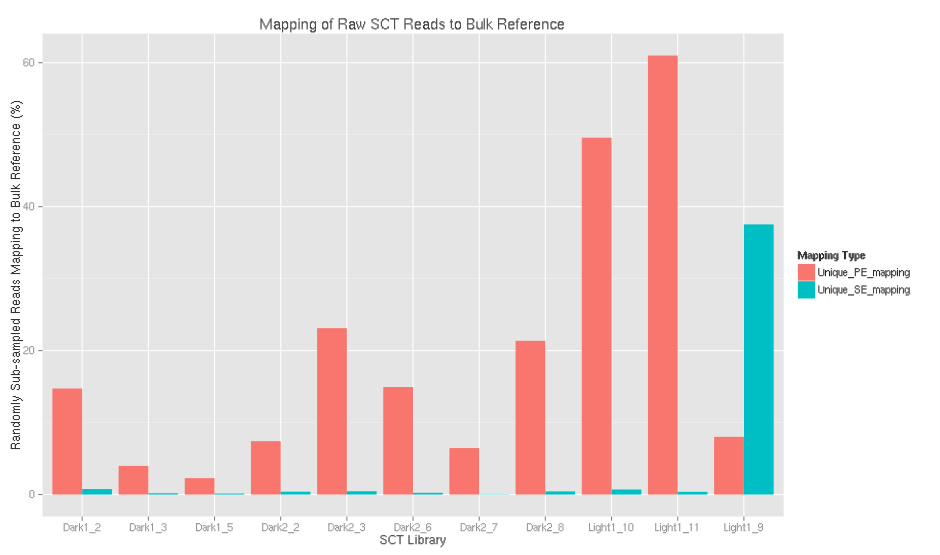
\includegraphics[width=\textwidth]{null_mapping.pdf}
    %plot of parameters random sampling and how they map 
    %null_mapping.svg
    %cutadapt vs trimmomatic plot
    \caption{Null mapping of 5000 randomly sampled PE reads from each SCT library 
                against a reference bulk transcriptome using bowtie2.
                %Of particular interest is the abnormal mapping of Light1\_9 library,
       %     where almost all reads map incongruently with their pair, despite bioanalyser
       %     traces showing fragment size selection with a clear peak at 360-385bp similarly
       % to the other libraries}
            }
    \label{fig:null_mapping}
\end{figure}




\begin{figure}[h]
    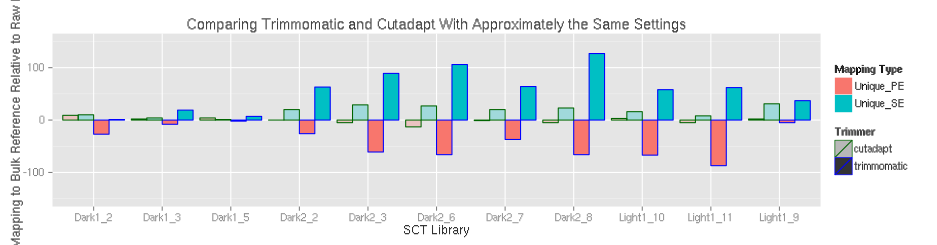
\includegraphics[width=\textwidth]{trimmomatic_vs_cutadapt.pdf}
    %plot of parameters random sampling and how they map 
    %null_mapping.svg
    %cutadapt vs trimmomatic plot
    \caption{Comparison of Trimmomatic and Cutadapt using approximately identical settings:
        specifically minimum length of 60, the entire contents of the Exeter Sequencing Service
        adapter file with respective error rate of 0.03 and Q15 for a simple match and an overall
        error threshold of Q30.

        Interestingly, cutadapt relatively increases the number of PE congruently mapping ends
        relative to untrimmed reads, whereas Trimmomatic generally leads to more PE reads mapping incongruently
        
        However, overall Trimmomatic with these settings has very slightly more paired reads mapping 
        181 vs 180.  

        The other advantages of Trimmomatic outweigh this slight performance deficit
    \label{fig:cvt}
\end{figure}



\begin{figure}[h]
    \includegraphis[width=\textwidth]{light9_insert_mapping.pdf}
\end{figure}


Scripts used to conduct this are available in my thesis scripts github repository:
\url{https://github.com/fmaguire/thesis_scripts/tree/master/chapter_2_assembly_and_binning/trimming_optimisation}


\subsubsection{Removing adaptors}

Optimising the trimmomatic settings.



Trimmomatic ILLUMINACLIP parameters: 

exeter_sequencing_adaptors.fasta

ILLUMINACLIP:/storage/fin/adapters/exeter_sequencing_adaptors.fasta:4:20:15
ILLUMINACLIP:/storage/fin/adapters/exeter_sequencing_adaptors.fasta:6:30:15
ILLUMINACLIP:/storage/fin/adapters/exeter_sequencing_adaptors.fasta:2:30:15
ILLUMINACLIP:/storage/fin/adapters/exeter_sequencing_adaptors.fasta:2:30:10
ILLUMINACLIP:/storage/fin/adapters/exeter_sequencing_adaptors.fasta:2:30:20

\subsubsection{Optimising Quality Thresholds}


\subsection{Library selection}
As assemblies were observed to considerably worsen or improve depending on the exact 
SCT library inclusion.  I sought to get a rough approximation for possible differences between
the libraries and to investigate possible contamination.  For this purpose, I created a tool
christened "DueyDrop".

To achieve this 5 batches of 10,000 PE reads were sampled from each library after trimming %which trim?
using seqtk's \citep{SeqtkGitHub} reservoir sampling algorithm with a common seed used to sample paired
reads for the forward and reverse read files for each PE library in the same manner as trimming optimisation.

While 5 batches of 10,000 should be equivalent to 50,000 random samples by splitting sampling and using
a different random seed each time the risk of poor implementation of this randomisation algorithm is 
somewhat offset and standard deviations can be easily calculated to assess consistency of later results.

These random samples were subsequently used to query the NCBI Protein NR database via BLASTX as implemented
in Diamond.  A tool optimised for efficient BLASTing of short reads against larger databases.

The top hit for each read was kept and the GIs extracted.  Subsequently, these GIs were used to query
a local taxdump of the NCBI taxonomy database via BioPerl.

These taxonomic data were then tallied at multiple taxonomic levels summarised below.




\begin{table}[h]
\begin{tabular}{@{}|l|l|llllll@{}}
\toprule
\textbf{SCT Library} & \textit{\textbf{PE}} & \multicolumn{1}{l|}{\textbf{Eukaryote}} & \multicolumn{1}{l|}{\textbf{Bacteria}} & \multicolumn{1}{l|}{\textbf{Alveolate}} & \multicolumn{1}{l|}{\textbf{Viridiplantae}} & \multicolumn{1}{l|}{} & \multicolumn{1}{l|}{\textbf{Total Hits}} \\ \cmidrule(r){1-6} \cmidrule(l){8-8} 
\textit{Light1-9}    & \textit{R1}          & \multicolumn{1}{l|}{51.89 +/- 0.45}     & \multicolumn{1}{l|}{9.37 +/- 0.26}     & \multicolumn{1}{l|}{25.15 +/-  0.71}    & \multicolumn{1}{l|}{7.45 +/- 0.33}          & \multicolumn{1}{l|}{} & 69.49 +/- 0.37                           \\ \cmidrule(lr){2-2}
                     & \textit{R2}          & 51.75 +/- 0.25                          & 8.82 +/- 0.24                          & 24.85 +/- 0.56                          & 7.49 +/- 0.21                               &                       & 68.75 +/- 0.29                           \\ \cmidrule(r){1-2}
\textit{Light1-10}   & \textit{R1}          &                                         &                                        &                                         & \multicolumn{1}{l|}{}                       & \multicolumn{1}{l|}{} &                                          \\ \cmidrule(lr){2-2}
                     & \textit{R2}          &                                         &                                        &                                         &                                             &                       &                                          \\ \cmidrule(r){1-2}
\textit{Light1-11}   & \textit{R1}          &                                         &                                        &                                         & \multicolumn{1}{l|}{}                       & \multicolumn{1}{l|}{} &                                          \\ \cmidrule(lr){2-2}
                     & \textit{R2}          &                                         &                                        &                                         &                                             &                       &                                          \\ \cmidrule(r){1-2}
\textit{Dark1-2}     & \textit{R1}          &                                         &                                        &                                         & \multicolumn{1}{l|}{}                       & \multicolumn{1}{l|}{} &                                          \\ \cmidrule(lr){2-2}
                     & \textit{R2}          &                                         &                                        &                                         &                                             &                       &                                          \\ \cmidrule(r){1-2}
\textit{Dark1-3}     & \textit{R1}          &                                         &                                        &                                         & \multicolumn{1}{l|}{}                       & \multicolumn{1}{l|}{} &                                          \\ \cmidrule(lr){2-2}
                     & \textit{R2}          &                                         &                                        &                                         &                                             &                       &                                          \\ \cmidrule(r){1-2}
\textit{Dark1-5}     & \textit{R1}          &                                         &                                        &                                         & \multicolumn{1}{l|}{}                       & \multicolumn{1}{l|}{} &                                          \\ \cmidrule(lr){2-2}
                     & \textit{R2}          &                                         &                                        &                                         &                                             &                       &                                          \\ \cmidrule(r){1-2}
\textit{Dark2-2}     & \textit{R1}          &                                         &                                        &                                         & \multicolumn{1}{l|}{}                       & \multicolumn{1}{l|}{} &                                          \\ \cmidrule(lr){2-2}
                     & \textit{R2}          &                                         &                                        &                                         &                                             &                       &                                          \\ \cmidrule(r){1-2}
\textit{Dark2-3}     & \textit{R1}          &                                         &                                        &                                         & \multicolumn{1}{l|}{}                       & \multicolumn{1}{l|}{} &                                          \\ \cmidrule(lr){2-2}
                     & \textit{R2}          &                                         &                                        &                                         &                                             &                       &                                          \\ \cmidrule(r){1-2}
\textit{Dark2-6}     & \textit{R1}          &                                         &                                        &                                         & \multicolumn{1}{l|}{}                       & \multicolumn{1}{l|}{} &                                          \\ \cmidrule(lr){2-2}
                     & \textit{R2}          &                                         &                                        &                                         &                                             &                       &                                          \\ \cmidrule(r){1-2}
\textit{Dark2-7}     & \textit{R1}          &                                         &                                        &                                         & \multicolumn{1}{l|}{}                       & \multicolumn{1}{l|}{} &                                          \\ \cmidrule(lr){2-2}
                     & \textit{R2}          &                                         &                                        &                                         &                                             &                       &                                          \\ \cmidrule(r){1-2}
\textit{Dark2-8}     & \textit{R1}          &                                         &                                        &                                         & \multicolumn{1}{l|}{}                       & \multicolumn{1}{l|}{} &                                          \\ \cmidrule(lr){2-2} \cmidrule(l){7-8} 
                     & \textit{R2}          &                                         &                                        &                                         &                                             &                       &                                          \\ \cmidrule(r){1-2}
\end{tabular}
\end{table}



Scripts used to conduct this are available in my thesis scripts github repository:
\url{https://github.com/fmaguire/dueydrop}

\subsection{GC Partitioning of Reads}
Paired Arrangement of Reads via K-means On Unlabelled Reads (parKour).

As we expect the metagenome to contain predominantly a highly AT-rich organism, \textit{Paramecium},
(ranging from 24.1 to 28.2\%GC in \textit{P. aurelia} species complex and \textit{P. caudatum} \citep{Aury2006,McGrath2014})
and a very GC-rich organism, \textit{Micractinium}, (\textit{Chlorella variabilis} NC64A genome is approximately 67.1\%GC, the highest
found in a sequenced eukaryote genome (in 2010) \citep{Blanc2010}).

Although intriguingly low-GC regions 55-65\%GC have a significantly higher number of mapped genes suggesting they are highly expressed \citep{Blanc2010}

Also correlations with increased GC richness in highly expressed regions of paramecium

Therefore,  would be closer than whole genome richness but still separable, this can be seen in the bimodal GC distribution in the raw and trimmed sequencing 
reads.

\begin{figure}
    Example GC plot showing bimodal distribution
\end{figure}

Due to the difficulties generating a high quality \textit{de novo} metatranscriptome assembly, I considered  it worth investigating whether there could be GC\%
clusters and furthermore whether assigning reads to these clusters and assembling the reads corresponding to a cluster would generate any meaningful groupings of reads.

To this end, I 

parKour:
\begin{enumerate}
    \item Parse user input of paired FASTQ files corresponding to Forward and Reverse Paired-End reads, and desired number of clusters
    \item Simultaneously iterate over the pair of FASTQ files calculating the GC\% for each loading results into an Armadillo \(2xN\) matrix where \(N\) is the total number of PE reads
    \item MLPACK K-means clustering:
        \begin{itemize}
            \item \
        \end{itemize}
    \item 
    \item Re-read the two input FASTQs assigning them to output files based on the assigned cluster of the pair
\end{enumerate}



Scripts used to conduct this are available in a github repository:
\url{https://github.com/fmaguire/parKour}



\subsection{Assembly}

Trinity uber alles

\subsubsection{Comparing assemblers}
Trinity,
SOAP de novo Trans
TransAbyss
Velvet+Oases

Trinity best

\subsubsection{Optimising Trinity Assembly}

minkmer cov 2: yay or nay

Error correction: yay or nay

Digital normalisation: yay or nay

\subsubsection{Assembly assessment}
RSEM-eval
Mapping percentage




\section{Binning}
For this purpose ete2 library was ported to python3 (pull request outstanding to merge this into ete2 codebase)
\subsection{Dendrogenous}
Phylogeny generation

\subsection{Arboretum}
Binner 

Training data manually parsed



\section{Saturation}
Estimating saturation can only be done after binning as we are only interested in host and algal endosymbiont
So saturation on binned contigs.



\section{Genome assembly}



Genome assembly - spades macmanes trimming was worse than spades harash trimming (shorter contigs)


